\documentclass[12pt,letterpaper]{article}
\usepackage[margin=0.65in,top=0.75in,bottom=0.65in,headheight=15pt,headsep=17pt,footskip=24pt]{geometry}
\usepackage{lmodern}
\pdfmapfile{+lm.map}
\pdfmapfile{+cm.map}
\usepackage{tikz}
\usetikzlibrary{arrows.meta}
\usepackage{fancyhdr}
\renewcommand{\familydefault}{\sfdefault}
\setlength{\parindent}{0pt}
\setlength{\parskip}{7pt}
\pagestyle{fancy}
\fancyhf{}
\renewcommand{\headrulewidth}{0pt}
\renewcommand{\footrulewidth}{0pt}
\fancyhead[L]{\fontsize{11}{13}\selectfont Week 13 / Route packing and bottlenecks / Grades 2--3}
\fancyfoot[L]{\fontsize{9}{11}\selectfont Bellingham Math Circle / Week 13 / F13-23-v2}
\fancyfoot[R]{\fontsize{9}{11}\selectfont\thepage}
\begin{document}
\fontsize{12}{16}\selectfont
A route follows arrows from Start to Finish without visiting a dot twice. Routes may meet at dots, but each arrow can belong to only one route in a collection. Use a different color or line pattern for each route. A marker closes one arrow.
\vspace{0.1in}
\par\textbf{Problem 1:} On each board, fit as many routes as possible. Find the fewest arrows you can close to stop every route.

\vspace{0.05in}
\begin{center}
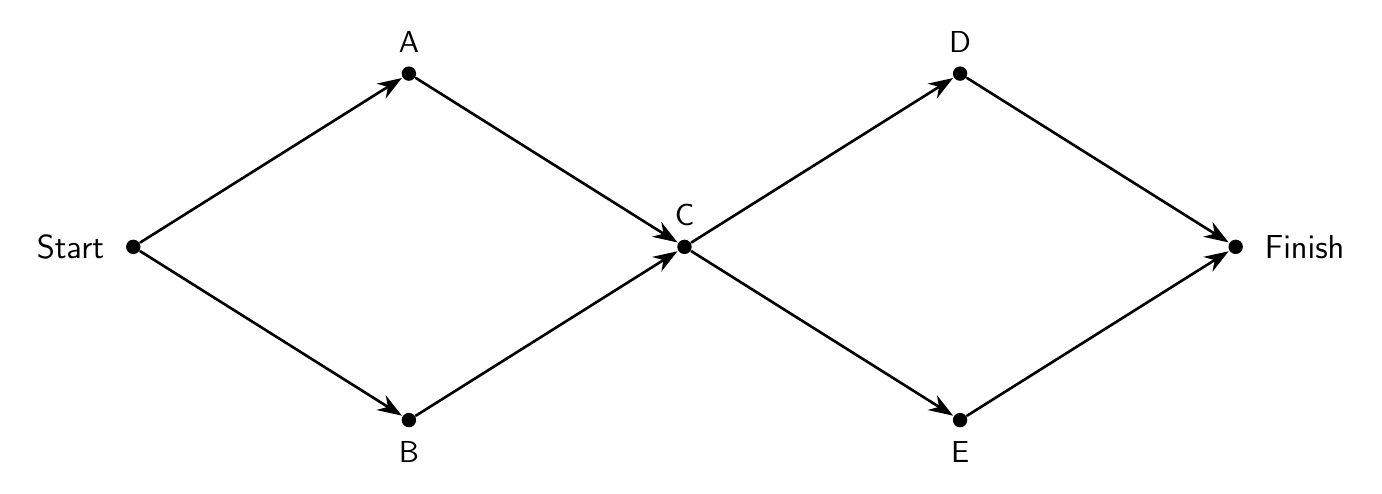
\begin{tikzpicture}[x=1cm,y=1cm,>={Stealth[length=3.1mm,width=2.2mm]},line cap=round,line join=round]
\coordinate (s) at (0,0);
\coordinate (A) at (3.5,2.2);
\coordinate (B) at (3.5,-2.2);
\coordinate (C) at (7,0);
\coordinate (D) at (10.5,2.2);
\coordinate (E) at (10.5,-2.2);
\coordinate (t) at (14,0);
\draw[->,line width=0.95pt,shorten >=3pt,shorten <=3pt] (s) -- (A);
\draw[->,line width=0.95pt,shorten >=3pt,shorten <=3pt] (s) -- (B);
\draw[->,line width=0.95pt,shorten >=3pt,shorten <=3pt] (A) -- (C);
\draw[->,line width=0.95pt,shorten >=3pt,shorten <=3pt] (B) -- (C);
\draw[->,line width=0.95pt,shorten >=3pt,shorten <=3pt] (C) -- (D);
\draw[->,line width=0.95pt,shorten >=3pt,shorten <=3pt] (C) -- (E);
\draw[->,line width=0.95pt,shorten >=3pt,shorten <=3pt] (D) -- (t);
\draw[->,line width=0.95pt,shorten >=3pt,shorten <=3pt] (E) -- (t);
\fill (s) circle (2.6pt);
\node[left=7pt,font=\fontsize{12}{14}\selectfont] at (s) {Start};
\fill (A) circle (2.6pt);
\node[above=6pt,fill=white,inner sep=1.4pt,font=\fontsize{11}{12}\selectfont] at (A) {A};
\fill (B) circle (2.6pt);
\node[below=6pt,fill=white,inner sep=1.4pt,font=\fontsize{11}{12}\selectfont] at (B) {B};
\fill (C) circle (2.6pt);
\node[above=6pt,fill=white,inner sep=1.4pt,font=\fontsize{11}{12}\selectfont] at (C) {C};
\fill (D) circle (2.6pt);
\node[above=6pt,fill=white,inner sep=1.4pt,font=\fontsize{11}{12}\selectfont] at (D) {D};
\fill (E) circle (2.6pt);
\node[below=6pt,fill=white,inner sep=1.4pt,font=\fontsize{11}{12}\selectfont] at (E) {E};
\fill (t) circle (2.6pt);
\node[right=7pt,font=\fontsize{12}{14}\selectfont] at (t) {Finish};
\end{tikzpicture}
\end{center}
\vspace{0.32in}
\begin{center}
\begin{tikzpicture}[x=1cm,y=1cm,>={Stealth[length=3.1mm,width=2.2mm]},line cap=round,line join=round]
\coordinate (s) at (0,0);
\coordinate (A) at (7,2.2);
\coordinate (B) at (7,-2.2);
\coordinate (t) at (14,0);
\draw[->,line width=0.95pt,shorten >=3pt,shorten <=3pt] (s) -- (A);
\draw[->,line width=0.95pt,shorten >=3pt,shorten <=3pt] (s) -- (B);
\draw[->,line width=0.95pt,shorten >=3pt,shorten <=3pt] (A) -- (B);
\draw[->,line width=0.95pt,shorten >=3pt,shorten <=3pt] (A) -- (t);
\draw[->,line width=0.95pt,shorten >=3pt,shorten <=3pt] (B) -- (t);
\fill (s) circle (2.6pt);
\node[left=7pt,font=\fontsize{12}{14}\selectfont] at (s) {Start};
\fill (A) circle (2.6pt);
\node[above=6pt,fill=white,inner sep=1.4pt,font=\fontsize{11}{12}\selectfont] at (A) {A};
\fill (B) circle (2.6pt);
\node[below=6pt,fill=white,inner sep=1.4pt,font=\fontsize{11}{12}\selectfont] at (B) {B};
\fill (t) circle (2.6pt);
\node[right=7pt,font=\fontsize{12}{14}\selectfont] at (t) {Finish};
\end{tikzpicture}
\end{center}


\newpage
\par\textbf{Problem 2:} Find the largest collection of routes on this board. Close as few arrows as possible to stop every route. Explain how you know your collection cannot be larger.

\vspace{0.26in}
\begin{center}
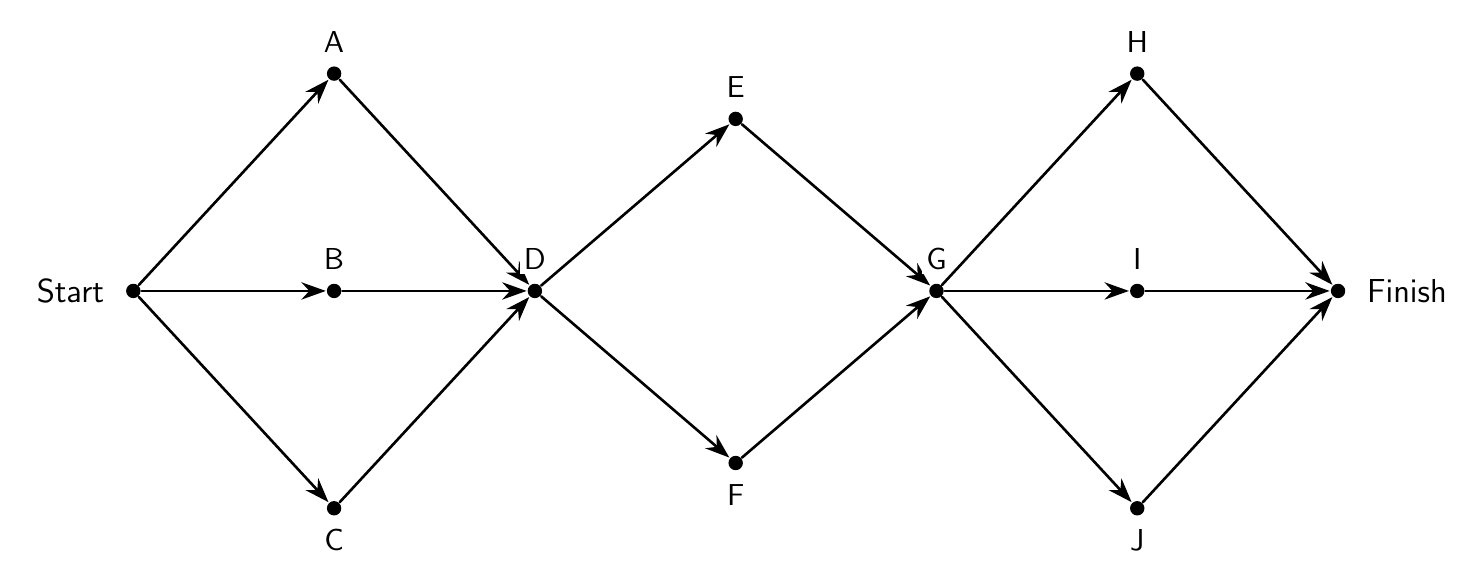
\begin{tikzpicture}[x=1.02cm,y=1.15cm,>={Stealth[length=3.1mm,width=2.2mm]},line cap=round,line join=round]
\coordinate (s) at (0,0);
\coordinate (A) at (2.5,2.4);
\coordinate (B) at (2.5,0);
\coordinate (C) at (2.5,-2.4);
\coordinate (D) at (5,0);
\coordinate (E) at (7.5,1.9);
\coordinate (F) at (7.5,-1.9);
\coordinate (G) at (10,0);
\coordinate (H) at (12.5,2.4);
\coordinate (I) at (12.5,0);
\coordinate (J) at (12.5,-2.4);
\coordinate (t) at (15,0);
\draw[->,line width=0.95pt,shorten >=3pt,shorten <=3pt] (s) -- (A);
\draw[->,line width=0.95pt,shorten >=3pt,shorten <=3pt] (s) -- (B);
\draw[->,line width=0.95pt,shorten >=3pt,shorten <=3pt] (s) -- (C);
\draw[->,line width=0.95pt,shorten >=3pt,shorten <=3pt] (A) -- (D);
\draw[->,line width=0.95pt,shorten >=3pt,shorten <=3pt] (B) -- (D);
\draw[->,line width=0.95pt,shorten >=3pt,shorten <=3pt] (C) -- (D);
\draw[->,line width=0.95pt,shorten >=3pt,shorten <=3pt] (D) -- (E);
\draw[->,line width=0.95pt,shorten >=3pt,shorten <=3pt] (D) -- (F);
\draw[->,line width=0.95pt,shorten >=3pt,shorten <=3pt] (E) -- (G);
\draw[->,line width=0.95pt,shorten >=3pt,shorten <=3pt] (F) -- (G);
\draw[->,line width=0.95pt,shorten >=3pt,shorten <=3pt] (G) -- (H);
\draw[->,line width=0.95pt,shorten >=3pt,shorten <=3pt] (G) -- (I);
\draw[->,line width=0.95pt,shorten >=3pt,shorten <=3pt] (G) -- (J);
\draw[->,line width=0.95pt,shorten >=3pt,shorten <=3pt] (H) -- (t);
\draw[->,line width=0.95pt,shorten >=3pt,shorten <=3pt] (I) -- (t);
\draw[->,line width=0.95pt,shorten >=3pt,shorten <=3pt] (J) -- (t);
\fill (s) circle (2.6pt);
\node[left=7pt,font=\fontsize{12}{14}\selectfont] at (s) {Start};
\fill (A) circle (2.6pt);
\node[above=6pt,fill=white,inner sep=1.4pt,font=\fontsize{11}{12}\selectfont] at (A) {A};
\fill (B) circle (2.6pt);
\node[above=6pt,fill=white,inner sep=1.4pt,font=\fontsize{11}{12}\selectfont] at (B) {B};
\fill (C) circle (2.6pt);
\node[below=6pt,fill=white,inner sep=1.4pt,font=\fontsize{11}{12}\selectfont] at (C) {C};
\fill (D) circle (2.6pt);
\node[above=6pt,fill=white,inner sep=1.4pt,font=\fontsize{11}{12}\selectfont] at (D) {D};
\fill (E) circle (2.6pt);
\node[above=6pt,fill=white,inner sep=1.4pt,font=\fontsize{11}{12}\selectfont] at (E) {E};
\fill (F) circle (2.6pt);
\node[below=6pt,fill=white,inner sep=1.4pt,font=\fontsize{11}{12}\selectfont] at (F) {F};
\fill (G) circle (2.6pt);
\node[above=6pt,fill=white,inner sep=1.4pt,font=\fontsize{11}{12}\selectfont] at (G) {G};
\fill (H) circle (2.6pt);
\node[above=6pt,fill=white,inner sep=1.4pt,font=\fontsize{11}{12}\selectfont] at (H) {H};
\fill (I) circle (2.6pt);
\node[above=6pt,fill=white,inner sep=1.4pt,font=\fontsize{11}{12}\selectfont] at (I) {I};
\fill (J) circle (2.6pt);
\node[below=6pt,fill=white,inner sep=1.4pt,font=\fontsize{11}{12}\selectfont] at (J) {J};
\fill (t) circle (2.6pt);
\node[right=7pt,font=\fontsize{12}{14}\selectfont] at (t) {Finish};
\end{tikzpicture}
\end{center}
\vspace{0.45in}

\newpage
\par\textbf{Problem 3:} Find every pair of arrows you can close to stop all travel on this board. Explain how you know your list is complete.

\vspace{0.26in}
\begin{center}
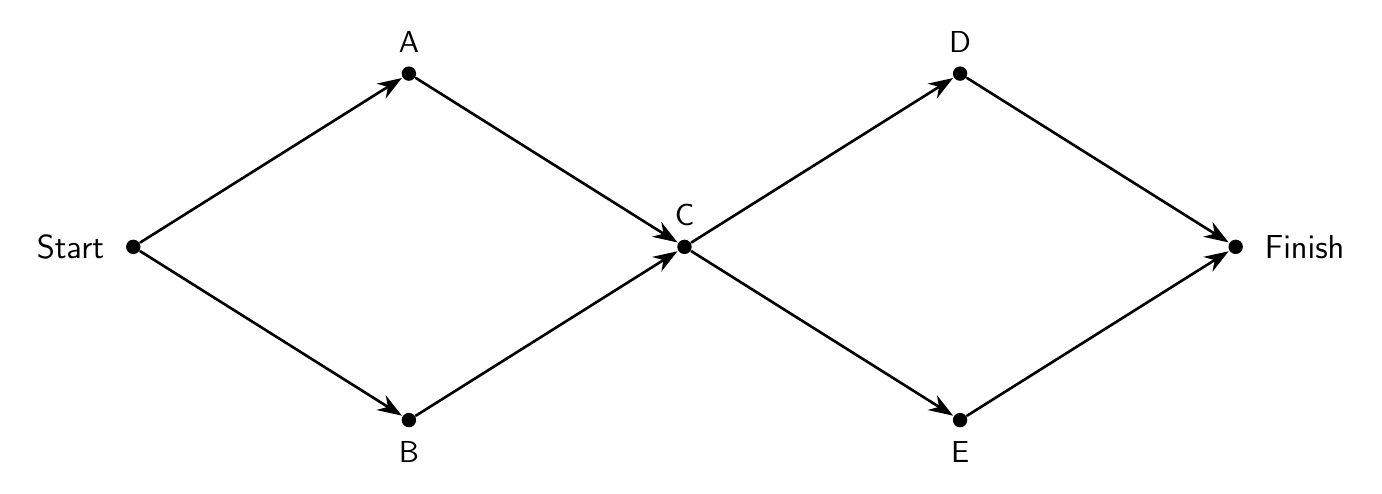
\begin{tikzpicture}[x=1cm,y=1cm,>={Stealth[length=3.1mm,width=2.2mm]},line cap=round,line join=round]
\coordinate (s) at (0,0);
\coordinate (A) at (3.5,2.2);
\coordinate (B) at (3.5,-2.2);
\coordinate (C) at (7,0);
\coordinate (D) at (10.5,2.2);
\coordinate (E) at (10.5,-2.2);
\coordinate (t) at (14,0);
\draw[->,line width=0.95pt,shorten >=3pt,shorten <=3pt] (s) -- (A);
\draw[->,line width=0.95pt,shorten >=3pt,shorten <=3pt] (s) -- (B);
\draw[->,line width=0.95pt,shorten >=3pt,shorten <=3pt] (A) -- (C);
\draw[->,line width=0.95pt,shorten >=3pt,shorten <=3pt] (B) -- (C);
\draw[->,line width=0.95pt,shorten >=3pt,shorten <=3pt] (C) -- (D);
\draw[->,line width=0.95pt,shorten >=3pt,shorten <=3pt] (C) -- (E);
\draw[->,line width=0.95pt,shorten >=3pt,shorten <=3pt] (D) -- (t);
\draw[->,line width=0.95pt,shorten >=3pt,shorten <=3pt] (E) -- (t);
\fill (s) circle (2.6pt);
\node[left=7pt,font=\fontsize{12}{14}\selectfont] at (s) {Start};
\fill (A) circle (2.6pt);
\node[above=6pt,fill=white,inner sep=1.4pt,font=\fontsize{11}{12}\selectfont] at (A) {A};
\fill (B) circle (2.6pt);
\node[below=6pt,fill=white,inner sep=1.4pt,font=\fontsize{11}{12}\selectfont] at (B) {B};
\fill (C) circle (2.6pt);
\node[above=6pt,fill=white,inner sep=1.4pt,font=\fontsize{11}{12}\selectfont] at (C) {C};
\fill (D) circle (2.6pt);
\node[above=6pt,fill=white,inner sep=1.4pt,font=\fontsize{11}{12}\selectfont] at (D) {D};
\fill (E) circle (2.6pt);
\node[below=6pt,fill=white,inner sep=1.4pt,font=\fontsize{11}{12}\selectfont] at (E) {E};
\fill (t) circle (2.6pt);
\node[right=7pt,font=\fontsize{12}{14}\selectfont] at (t) {Finish};
\end{tikzpicture}
\end{center}
\vspace{0.3in}

\newpage
\par\textbf{Problem 4:} On each board, add one new arrow between two inside dots so that three routes fit. The new arrow cannot touch Start or Finish. Crossings without a dot are not meeting points. If it is impossible, explain why.

\vspace{0.26in}
\begin{center}
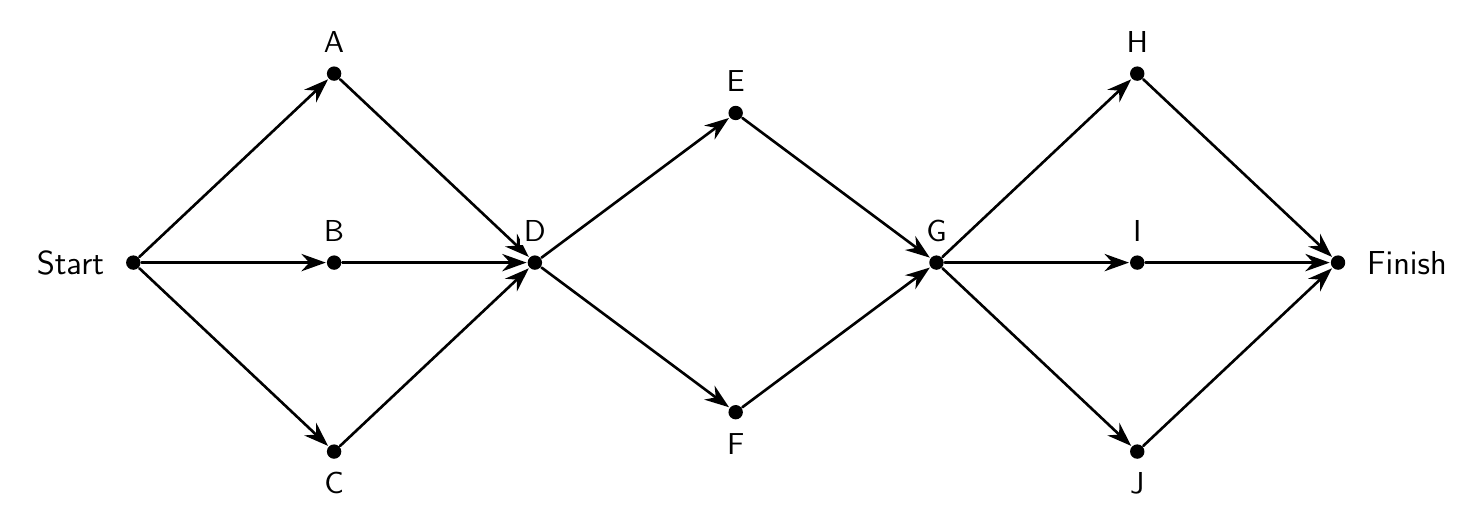
\begin{tikzpicture}[x=1.02cm,y=1cm,>={Stealth[length=3.1mm,width=2.2mm]},line cap=round,line join=round]
\coordinate (s) at (0,0);
\coordinate (A) at (2.5,2.4);
\coordinate (B) at (2.5,0);
\coordinate (C) at (2.5,-2.4);
\coordinate (D) at (5,0);
\coordinate (E) at (7.5,1.9);
\coordinate (F) at (7.5,-1.9);
\coordinate (G) at (10,0);
\coordinate (H) at (12.5,2.4);
\coordinate (I) at (12.5,0);
\coordinate (J) at (12.5,-2.4);
\coordinate (t) at (15,0);
\draw[->,line width=0.95pt,shorten >=3pt,shorten <=3pt] (s) -- (A);
\draw[->,line width=0.95pt,shorten >=3pt,shorten <=3pt] (s) -- (B);
\draw[->,line width=0.95pt,shorten >=3pt,shorten <=3pt] (s) -- (C);
\draw[->,line width=0.95pt,shorten >=3pt,shorten <=3pt] (A) -- (D);
\draw[->,line width=0.95pt,shorten >=3pt,shorten <=3pt] (B) -- (D);
\draw[->,line width=0.95pt,shorten >=3pt,shorten <=3pt] (C) -- (D);
\draw[->,line width=0.95pt,shorten >=3pt,shorten <=3pt] (D) -- (E);
\draw[->,line width=0.95pt,shorten >=3pt,shorten <=3pt] (D) -- (F);
\draw[->,line width=0.95pt,shorten >=3pt,shorten <=3pt] (E) -- (G);
\draw[->,line width=0.95pt,shorten >=3pt,shorten <=3pt] (F) -- (G);
\draw[->,line width=0.95pt,shorten >=3pt,shorten <=3pt] (G) -- (H);
\draw[->,line width=0.95pt,shorten >=3pt,shorten <=3pt] (G) -- (I);
\draw[->,line width=0.95pt,shorten >=3pt,shorten <=3pt] (G) -- (J);
\draw[->,line width=0.95pt,shorten >=3pt,shorten <=3pt] (H) -- (t);
\draw[->,line width=0.95pt,shorten >=3pt,shorten <=3pt] (I) -- (t);
\draw[->,line width=0.95pt,shorten >=3pt,shorten <=3pt] (J) -- (t);
\fill (s) circle (2.6pt);
\node[left=7pt,font=\fontsize{12}{14}\selectfont] at (s) {Start};
\fill (A) circle (2.6pt);
\node[above=6pt,fill=white,inner sep=1.4pt,font=\fontsize{11}{12}\selectfont] at (A) {A};
\fill (B) circle (2.6pt);
\node[above=6pt,fill=white,inner sep=1.4pt,font=\fontsize{11}{12}\selectfont] at (B) {B};
\fill (C) circle (2.6pt);
\node[below=6pt,fill=white,inner sep=1.4pt,font=\fontsize{11}{12}\selectfont] at (C) {C};
\fill (D) circle (2.6pt);
\node[above=6pt,fill=white,inner sep=1.4pt,font=\fontsize{11}{12}\selectfont] at (D) {D};
\fill (E) circle (2.6pt);
\node[above=6pt,fill=white,inner sep=1.4pt,font=\fontsize{11}{12}\selectfont] at (E) {E};
\fill (F) circle (2.6pt);
\node[below=6pt,fill=white,inner sep=1.4pt,font=\fontsize{11}{12}\selectfont] at (F) {F};
\fill (G) circle (2.6pt);
\node[above=6pt,fill=white,inner sep=1.4pt,font=\fontsize{11}{12}\selectfont] at (G) {G};
\fill (H) circle (2.6pt);
\node[above=6pt,fill=white,inner sep=1.4pt,font=\fontsize{11}{12}\selectfont] at (H) {H};
\fill (I) circle (2.6pt);
\node[above=6pt,fill=white,inner sep=1.4pt,font=\fontsize{11}{12}\selectfont] at (I) {I};
\fill (J) circle (2.6pt);
\node[below=6pt,fill=white,inner sep=1.4pt,font=\fontsize{11}{12}\selectfont] at (J) {J};
\fill (t) circle (2.6pt);
\node[right=7pt,font=\fontsize{12}{14}\selectfont] at (t) {Finish};
\end{tikzpicture}
\end{center}
\vspace{0.32in}
\begin{center}
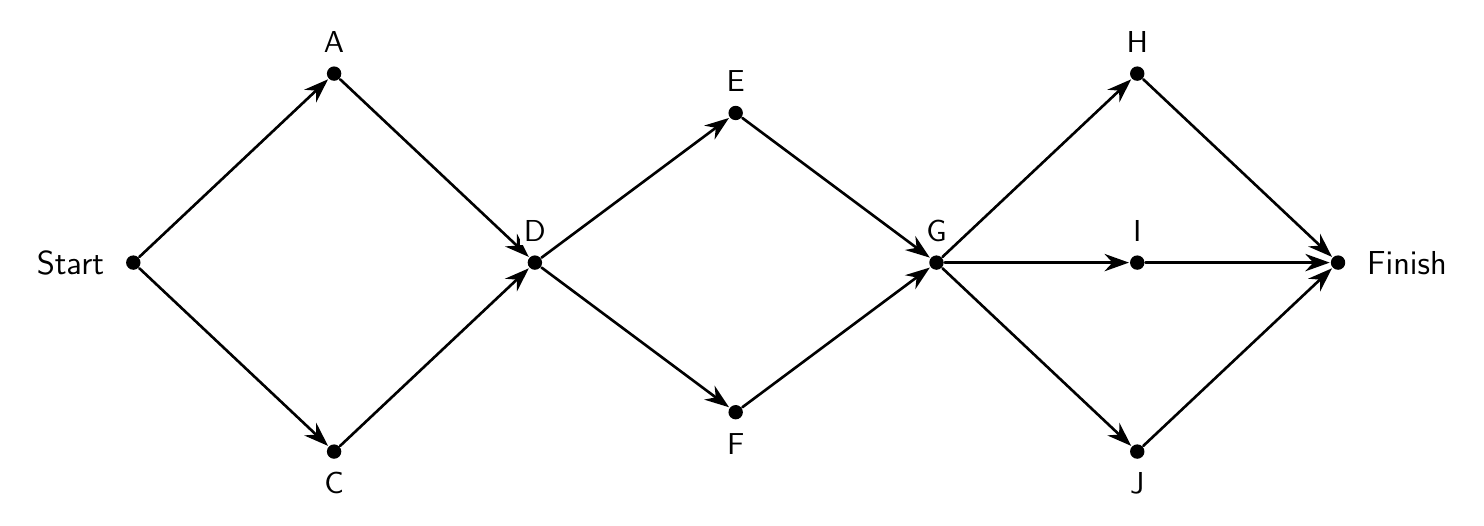
\begin{tikzpicture}[x=1.02cm,y=1cm,>={Stealth[length=3.1mm,width=2.2mm]},line cap=round,line join=round]
\coordinate (s) at (0,0);
\coordinate (A) at (2.5,2.4);
\coordinate (C) at (2.5,-2.4);
\coordinate (D) at (5,0);
\coordinate (E) at (7.5,1.9);
\coordinate (F) at (7.5,-1.9);
\coordinate (G) at (10,0);
\coordinate (H) at (12.5,2.4);
\coordinate (I) at (12.5,0);
\coordinate (J) at (12.5,-2.4);
\coordinate (t) at (15,0);
\draw[->,line width=0.95pt,shorten >=3pt,shorten <=3pt] (s) -- (A);
\draw[->,line width=0.95pt,shorten >=3pt,shorten <=3pt] (s) -- (C);
\draw[->,line width=0.95pt,shorten >=3pt,shorten <=3pt] (A) -- (D);
\draw[->,line width=0.95pt,shorten >=3pt,shorten <=3pt] (C) -- (D);
\draw[->,line width=0.95pt,shorten >=3pt,shorten <=3pt] (D) -- (E);
\draw[->,line width=0.95pt,shorten >=3pt,shorten <=3pt] (D) -- (F);
\draw[->,line width=0.95pt,shorten >=3pt,shorten <=3pt] (E) -- (G);
\draw[->,line width=0.95pt,shorten >=3pt,shorten <=3pt] (F) -- (G);
\draw[->,line width=0.95pt,shorten >=3pt,shorten <=3pt] (G) -- (H);
\draw[->,line width=0.95pt,shorten >=3pt,shorten <=3pt] (G) -- (I);
\draw[->,line width=0.95pt,shorten >=3pt,shorten <=3pt] (G) -- (J);
\draw[->,line width=0.95pt,shorten >=3pt,shorten <=3pt] (H) -- (t);
\draw[->,line width=0.95pt,shorten >=3pt,shorten <=3pt] (I) -- (t);
\draw[->,line width=0.95pt,shorten >=3pt,shorten <=3pt] (J) -- (t);
\fill (s) circle (2.6pt);
\node[left=7pt,font=\fontsize{12}{14}\selectfont] at (s) {Start};
\fill (A) circle (2.6pt);
\node[above=6pt,fill=white,inner sep=1.4pt,font=\fontsize{11}{12}\selectfont] at (A) {A};
\fill (C) circle (2.6pt);
\node[below=6pt,fill=white,inner sep=1.4pt,font=\fontsize{11}{12}\selectfont] at (C) {C};
\fill (D) circle (2.6pt);
\node[above=6pt,fill=white,inner sep=1.4pt,font=\fontsize{11}{12}\selectfont] at (D) {D};
\fill (E) circle (2.6pt);
\node[above=6pt,fill=white,inner sep=1.4pt,font=\fontsize{11}{12}\selectfont] at (E) {E};
\fill (F) circle (2.6pt);
\node[below=6pt,fill=white,inner sep=1.4pt,font=\fontsize{11}{12}\selectfont] at (F) {F};
\fill (G) circle (2.6pt);
\node[above=6pt,fill=white,inner sep=1.4pt,font=\fontsize{11}{12}\selectfont] at (G) {G};
\fill (H) circle (2.6pt);
\node[above=6pt,fill=white,inner sep=1.4pt,font=\fontsize{11}{12}\selectfont] at (H) {H};
\fill (I) circle (2.6pt);
\node[above=6pt,fill=white,inner sep=1.4pt,font=\fontsize{11}{12}\selectfont] at (I) {I};
\fill (J) circle (2.6pt);
\node[below=6pt,fill=white,inner sep=1.4pt,font=\fontsize{11}{12}\selectfont] at (J) {J};
\fill (t) circle (2.6pt);
\node[right=7pt,font=\fontsize{12}{14}\selectfont] at (t) {Finish};
\end{tikzpicture}
\end{center}


\newpage
\par\textbf{Problem 5:} The thick arrows form reserved routes. No more routes fit beside them. Replace them with a largest collection on each board.

\vspace{0.26in}
\begin{center}
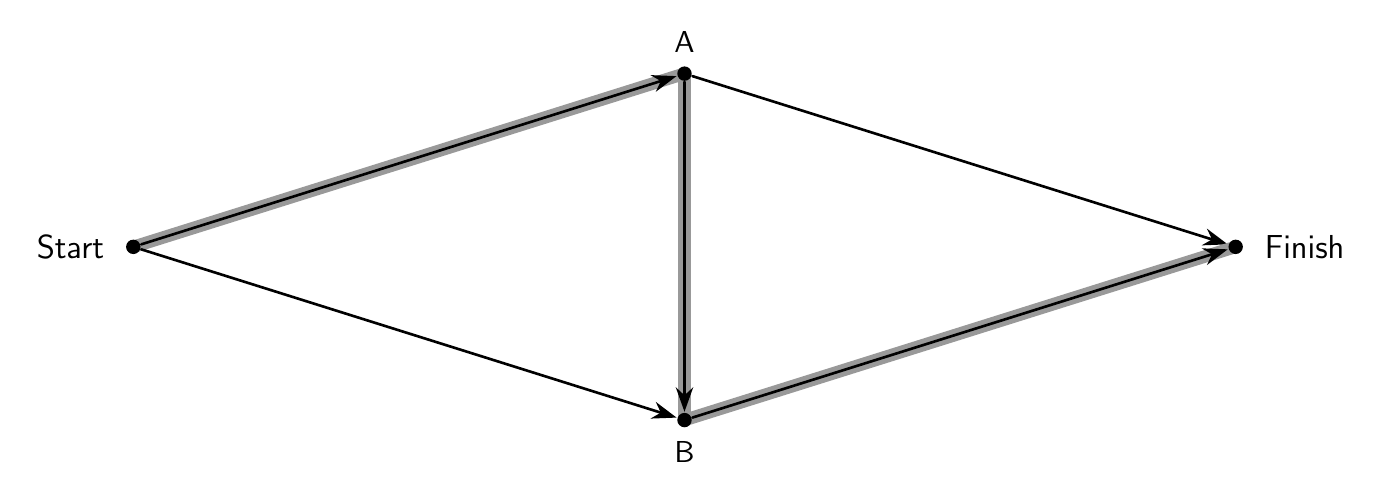
\begin{tikzpicture}[x=1cm,y=1cm,>={Stealth[length=3.1mm,width=2.2mm]},line cap=round,line join=round]
\coordinate (s) at (0,0);
\coordinate (A) at (7,2.2);
\coordinate (B) at (7,-2.2);
\coordinate (t) at (14,0);
\draw[line width=4.5pt,black!40] (s) -- (A);
\draw[->,line width=0.95pt,shorten >=3pt,shorten <=3pt] (s) -- (A);
\draw[->,line width=0.95pt,shorten >=3pt,shorten <=3pt] (s) -- (B);
\draw[line width=4.5pt,black!40] (A) -- (B);
\draw[->,line width=0.95pt,shorten >=3pt,shorten <=3pt] (A) -- (B);
\draw[->,line width=0.95pt,shorten >=3pt,shorten <=3pt] (A) -- (t);
\draw[line width=4.5pt,black!40] (B) -- (t);
\draw[->,line width=0.95pt,shorten >=3pt,shorten <=3pt] (B) -- (t);
\fill (s) circle (2.6pt);
\node[left=7pt,font=\fontsize{12}{14}\selectfont] at (s) {Start};
\fill (A) circle (2.6pt);
\node[above=6pt,fill=white,inner sep=1.4pt,font=\fontsize{11}{12}\selectfont] at (A) {A};
\fill (B) circle (2.6pt);
\node[below=6pt,fill=white,inner sep=1.4pt,font=\fontsize{11}{12}\selectfont] at (B) {B};
\fill (t) circle (2.6pt);
\node[right=7pt,font=\fontsize{12}{14}\selectfont] at (t) {Finish};
\end{tikzpicture}
\end{center}
\vspace{0.32in}
\begin{center}
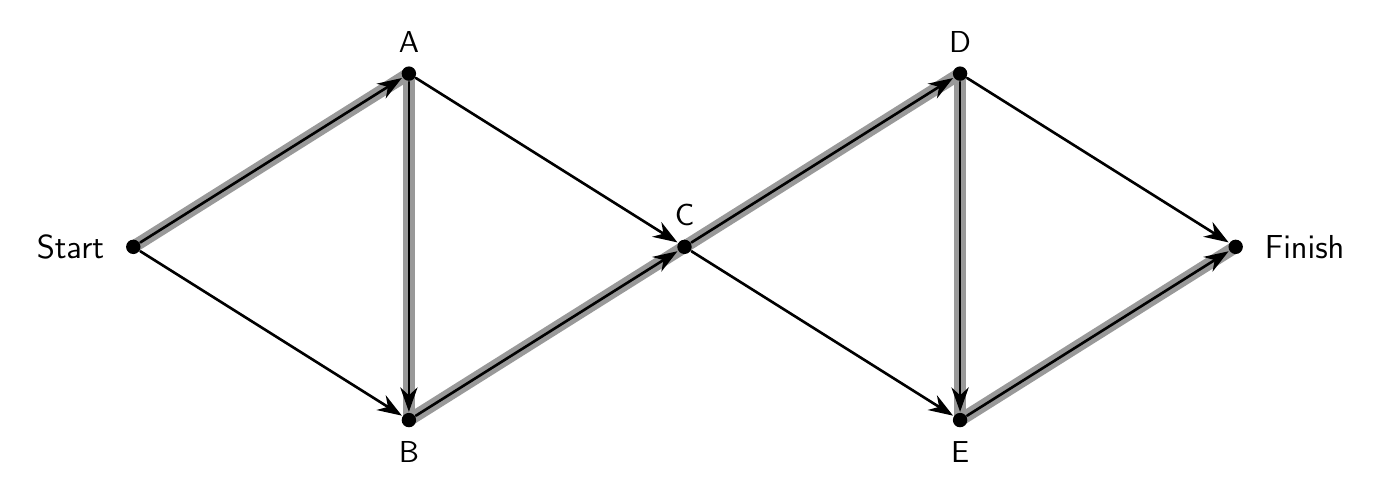
\begin{tikzpicture}[x=1cm,y=1cm,>={Stealth[length=3.1mm,width=2.2mm]},line cap=round,line join=round]
\coordinate (s) at (0,0);
\coordinate (A) at (3.5,2.2);
\coordinate (B) at (3.5,-2.2);
\coordinate (C) at (7,0);
\coordinate (D) at (10.5,2.2);
\coordinate (E) at (10.5,-2.2);
\coordinate (t) at (14,0);
\draw[line width=4.5pt,black!40] (s) -- (A);
\draw[->,line width=0.95pt,shorten >=3pt,shorten <=3pt] (s) -- (A);
\draw[->,line width=0.95pt,shorten >=3pt,shorten <=3pt] (s) -- (B);
\draw[line width=4.5pt,black!40] (A) -- (B);
\draw[->,line width=0.95pt,shorten >=3pt,shorten <=3pt] (A) -- (B);
\draw[->,line width=0.95pt,shorten >=3pt,shorten <=3pt] (A) -- (C);
\draw[line width=4.5pt,black!40] (B) -- (C);
\draw[->,line width=0.95pt,shorten >=3pt,shorten <=3pt] (B) -- (C);
\draw[line width=4.5pt,black!40] (C) -- (D);
\draw[->,line width=0.95pt,shorten >=3pt,shorten <=3pt] (C) -- (D);
\draw[->,line width=0.95pt,shorten >=3pt,shorten <=3pt] (C) -- (E);
\draw[line width=4.5pt,black!40] (D) -- (E);
\draw[->,line width=0.95pt,shorten >=3pt,shorten <=3pt] (D) -- (E);
\draw[->,line width=0.95pt,shorten >=3pt,shorten <=3pt] (D) -- (t);
\draw[line width=4.5pt,black!40] (E) -- (t);
\draw[->,line width=0.95pt,shorten >=3pt,shorten <=3pt] (E) -- (t);
\fill (s) circle (2.6pt);
\node[left=7pt,font=\fontsize{12}{14}\selectfont] at (s) {Start};
\fill (A) circle (2.6pt);
\node[above=6pt,fill=white,inner sep=1.4pt,font=\fontsize{11}{12}\selectfont] at (A) {A};
\fill (B) circle (2.6pt);
\node[below=6pt,fill=white,inner sep=1.4pt,font=\fontsize{11}{12}\selectfont] at (B) {B};
\fill (C) circle (2.6pt);
\node[above=6pt,fill=white,inner sep=1.4pt,font=\fontsize{11}{12}\selectfont] at (C) {C};
\fill (D) circle (2.6pt);
\node[above=6pt,fill=white,inner sep=1.4pt,font=\fontsize{11}{12}\selectfont] at (D) {D};
\fill (E) circle (2.6pt);
\node[below=6pt,fill=white,inner sep=1.4pt,font=\fontsize{11}{12}\selectfont] at (E) {E};
\fill (t) circle (2.6pt);
\node[right=7pt,font=\fontsize{12}{14}\selectfont] at (t) {Finish};
\end{tikzpicture}
\end{center}


\newpage

\vspace{0.05in}
\begin{center}
\begin{tikzpicture}[x=1cm,y=1cm,>={Stealth[length=3.1mm,width=2.2mm]},line cap=round,line join=round]
\coordinate (s) at (0,0);
\coordinate (A) at (7,2.2);
\coordinate (B) at (7,-2.2);
\coordinate (t) at (14,0);
\draw[->,line width=0.95pt,shorten >=3pt,shorten <=3pt] (s) -- (A);
\draw[->,line width=0.95pt,shorten >=3pt,shorten <=3pt] (s) -- (B);
\draw[->,line width=0.95pt,shorten >=3pt,shorten <=3pt] (A) -- (B);
\draw[->,line width=0.95pt,shorten >=3pt,shorten <=3pt] (A) -- (t);
\draw[->,line width=0.95pt,shorten >=3pt,shorten <=3pt] (B) -- (t);
\fill (s) circle (2.6pt);
\node[left=7pt,font=\fontsize{12}{14}\selectfont] at (s) {Start};
\fill (A) circle (2.6pt);
\node[above=6pt,fill=white,inner sep=1.4pt,font=\fontsize{11}{12}\selectfont] at (A) {A};
\fill (B) circle (2.6pt);
\node[below=6pt,fill=white,inner sep=1.4pt,font=\fontsize{11}{12}\selectfont] at (B) {B};
\fill (t) circle (2.6pt);
\node[right=7pt,font=\fontsize{12}{14}\selectfont] at (t) {Finish};
\end{tikzpicture}
\end{center}
\vspace{0.32in}
\begin{center}
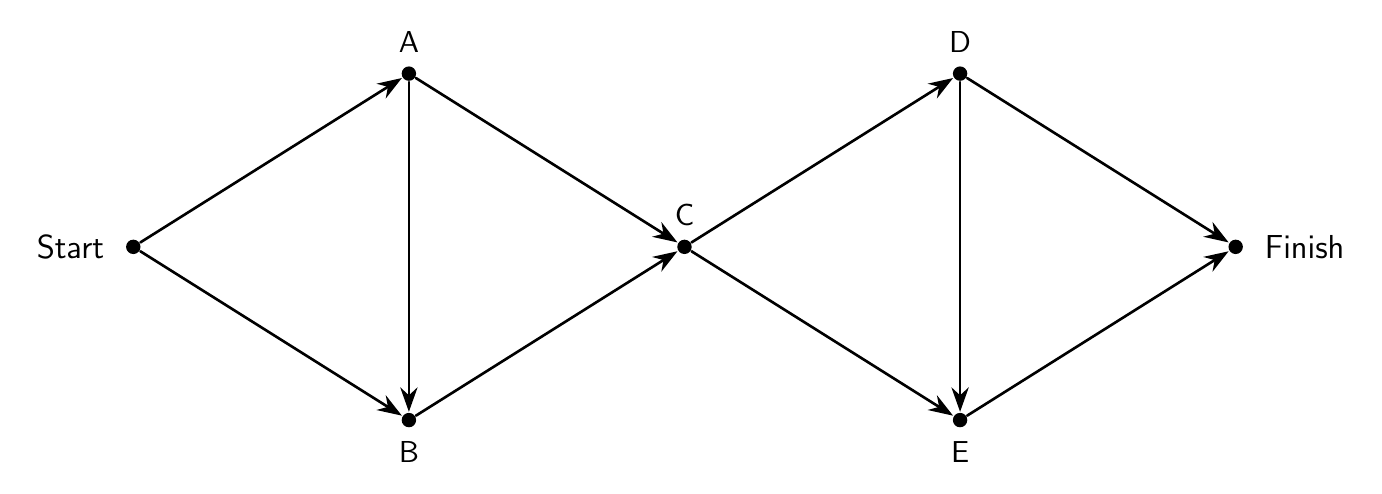
\begin{tikzpicture}[x=1cm,y=1cm,>={Stealth[length=3.1mm,width=2.2mm]},line cap=round,line join=round]
\coordinate (s) at (0,0);
\coordinate (A) at (3.5,2.2);
\coordinate (B) at (3.5,-2.2);
\coordinate (C) at (7,0);
\coordinate (D) at (10.5,2.2);
\coordinate (E) at (10.5,-2.2);
\coordinate (t) at (14,0);
\draw[->,line width=0.95pt,shorten >=3pt,shorten <=3pt] (s) -- (A);
\draw[->,line width=0.95pt,shorten >=3pt,shorten <=3pt] (s) -- (B);
\draw[->,line width=0.95pt,shorten >=3pt,shorten <=3pt] (A) -- (B);
\draw[->,line width=0.95pt,shorten >=3pt,shorten <=3pt] (A) -- (C);
\draw[->,line width=0.95pt,shorten >=3pt,shorten <=3pt] (B) -- (C);
\draw[->,line width=0.95pt,shorten >=3pt,shorten <=3pt] (C) -- (D);
\draw[->,line width=0.95pt,shorten >=3pt,shorten <=3pt] (C) -- (E);
\draw[->,line width=0.95pt,shorten >=3pt,shorten <=3pt] (D) -- (E);
\draw[->,line width=0.95pt,shorten >=3pt,shorten <=3pt] (D) -- (t);
\draw[->,line width=0.95pt,shorten >=3pt,shorten <=3pt] (E) -- (t);
\fill (s) circle (2.6pt);
\node[left=7pt,font=\fontsize{12}{14}\selectfont] at (s) {Start};
\fill (A) circle (2.6pt);
\node[above=6pt,fill=white,inner sep=1.4pt,font=\fontsize{11}{12}\selectfont] at (A) {A};
\fill (B) circle (2.6pt);
\node[below=6pt,fill=white,inner sep=1.4pt,font=\fontsize{11}{12}\selectfont] at (B) {B};
\fill (C) circle (2.6pt);
\node[above=6pt,fill=white,inner sep=1.4pt,font=\fontsize{11}{12}\selectfont] at (C) {C};
\fill (D) circle (2.6pt);
\node[above=6pt,fill=white,inner sep=1.4pt,font=\fontsize{11}{12}\selectfont] at (D) {D};
\fill (E) circle (2.6pt);
\node[below=6pt,fill=white,inner sep=1.4pt,font=\fontsize{11}{12}\selectfont] at (E) {E};
\fill (t) circle (2.6pt);
\node[right=7pt,font=\fontsize{12}{14}\selectfont] at (t) {Finish};
\end{tikzpicture}
\end{center}


\newpage
\par\textbf{Problem 6:} Two players take turns closing one open arrow. The player whose move leaves no route wins. Decide who can force a win on each board, and explain a strategy.

\vspace{0.26in}
\begin{center}
\begin{tikzpicture}[x=1cm,y=1cm,>={Stealth[length=3.1mm,width=2.2mm]},line cap=round,line join=round]
\coordinate (s) at (0,0);
\coordinate (A) at (7,2.2);
\coordinate (B) at (7,-2.2);
\coordinate (t) at (14,0);
\draw[->,line width=0.95pt,shorten >=3pt,shorten <=3pt] (s) -- (A);
\draw[->,line width=0.95pt,shorten >=3pt,shorten <=3pt] (s) -- (B);
\draw[->,line width=0.95pt,shorten >=3pt,shorten <=3pt] (A) -- (t);
\draw[->,line width=0.95pt,shorten >=3pt,shorten <=3pt] (B) -- (t);
\fill (s) circle (2.6pt);
\node[left=7pt,font=\fontsize{12}{14}\selectfont] at (s) {Start};
\fill (A) circle (2.6pt);
\node[above=6pt,fill=white,inner sep=1.4pt,font=\fontsize{11}{12}\selectfont] at (A) {A};
\fill (B) circle (2.6pt);
\node[below=6pt,fill=white,inner sep=1.4pt,font=\fontsize{11}{12}\selectfont] at (B) {B};
\fill (t) circle (2.6pt);
\node[right=7pt,font=\fontsize{12}{14}\selectfont] at (t) {Finish};
\end{tikzpicture}
\end{center}
\vspace{0.32in}
\begin{center}
\begin{tikzpicture}[x=1cm,y=1cm,>={Stealth[length=3.1mm,width=2.2mm]},line cap=round,line join=round]
\coordinate (s) at (0,0);
\coordinate (A) at (7,2.2);
\coordinate (B) at (7,-2.2);
\coordinate (t) at (14,0);
\draw[->,line width=0.95pt,shorten >=3pt,shorten <=3pt] (s) -- (A);
\draw[->,line width=0.95pt,shorten >=3pt,shorten <=3pt] (s) -- (B);
\draw[->,line width=0.95pt,shorten >=3pt,shorten <=3pt] (A) -- (B);
\draw[->,line width=0.95pt,shorten >=3pt,shorten <=3pt] (A) -- (t);
\draw[->,line width=0.95pt,shorten >=3pt,shorten <=3pt] (B) -- (t);
\fill (s) circle (2.6pt);
\node[left=7pt,font=\fontsize{12}{14}\selectfont] at (s) {Start};
\fill (A) circle (2.6pt);
\node[above=6pt,fill=white,inner sep=1.4pt,font=\fontsize{11}{12}\selectfont] at (A) {A};
\fill (B) circle (2.6pt);
\node[below=6pt,fill=white,inner sep=1.4pt,font=\fontsize{11}{12}\selectfont] at (B) {B};
\fill (t) circle (2.6pt);
\node[right=7pt,font=\fontsize{12}{14}\selectfont] at (t) {Finish};
\end{tikzpicture}
\end{center}


\end{document}
